% Keyboard Layouts
% Version 0.2
% (C) 2024-2025 Frank Hofmann <info@efho.de>
% Available from https://github.com/hofmannedv/cheatsheets

% Published under Creative Commons CC-BY-SA 4.0 International License
% https://creativecommons.org/licenses/by-sa/4.0/

\documentclass[10pt,a4paper]{article}
\usepackage{cheatsheeta4}

\renewcommand{\cheatsheetTitle}{Aide-mémoire du clavier}
\renewcommand{\cheatsheetVersion}{Version 0.2}
\renewcommand{\cheatsheetCopyright}{
  \copyright~ 2024-2025 Frank Hofmann \faIcon{envelope} \href{mailto:info@efho.de}{info@efho.de}~. Publié sous licence 
 \href{https://creativecommons.org/licenses/by-sa/4.0/}{Creative Commons CC-BY-SA 4.0 International License}. Créé avec \LaTeX. \\ \faIcon{github} \href{https://github.com/hofmannedv/cheatsheets}{https://github.com/hofmannedv/cheatsheets}~.\\
 Les illustrations sont tirées de Wikimedia: \href{https://commons.wikimedia.org/wiki/File:KB_United_States-NoAltGr.svg}{US Keyboard},
 \href{https://commons.wikimedia.org/wiki/File:KB_US-International.svg}{US International Keyboard}~, et \href{https://commons.wikimedia.org/wiki/File:KB_United_States_Mac_-_Apple_Keyboard_(MC184LL).svg}{US Keyboard Apple/Mac}. Les trois ont été publiés sous \href{https://creativecommons.org/licenses/by-sa/3.0/deed.en}{Creative Commons Attribution-Share Alike 3.0 Unported License}.
}

% add document metadata as XMP data
% add keywords based on hyperref package
\usepackage{hyperxmp}
\hypersetup{
    pdfauthor={Frank Hofmann}, 
    pdftitle={disposition du clavier},
    pdfkeywords={disposition du clavier, keyboard, États-Unis},
    pdfsubject={Disposition du clavier des États-Unis},
    pdfcopyright={Copyright (C) 2024-2025 Frank Hofmann. Publié sous licence Creative Commons Attribution - Share Alike 4.0 International License (CC-BY-SA-4.0)}
    pdfcopyrighturl={https://creativecommons.org/licenses/by-sa/4.0/legalcode.fr}
}

\begin{document}

\cheatsheet

\section{Disposition du clavier États-Unis (US Keyboard)}
\begin{center}
  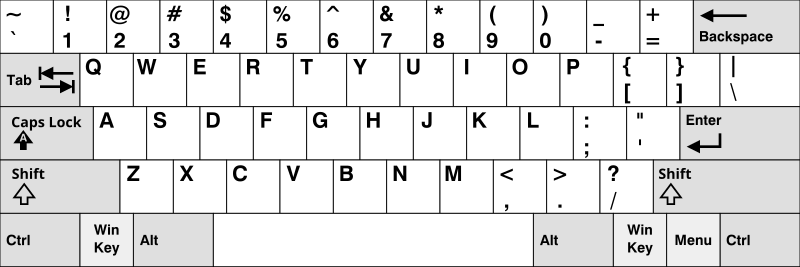
\includegraphics[height=5cm]{us.png}
\end{center}

\section{Disposition du clavier États-Unis International (US International Keyboard)}
\begin{center}
  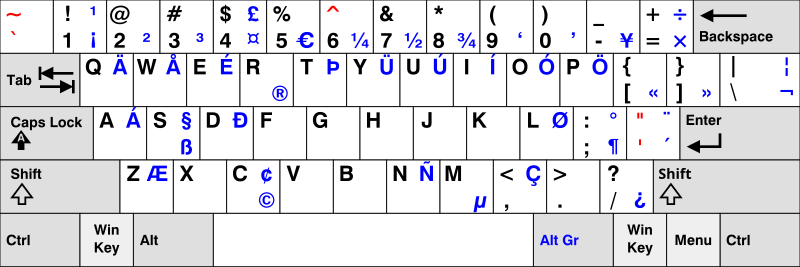
\includegraphics[height=5cm]{us-international.png}
\end{center}

\newpage
\cheatsheet

\section{Disposition du clavier États-Unis Apple (US Keyboard Apple/Mac)}
\begin{center}
  \includegraphics[height=5cm]{us-apple.png}
\end{center}

\end{document}
